\documentclass[11pt]{article}

\usepackage{graphicx}

% Enable references to labels in the notes
\usepackage{xr-hyper}
\externaldocument{p328_notes}
\usepackage{hyperref}

% Sans fonts
\usepackage{sfmath}
\renewcommand{\familydefault}{\sfdefault}

\newcommand{\COURSE}{PHYS328W}
\newcommand{\LABNUM}{4}
\newcommand{\TITLE}{An RLC Filter}
\markright{\COURSE~Lab \LABNUM\ : \TITLE}

\setlength{\textwidth} {6.5 true in}
\setlength{\textheight}{9 true in}
\setlength{\hoffset}   {-0.75 true in}
\setlength{\voffset}   {-0.75 true in}
\setlength{\parindent} {12 pt}
\pagestyle{myheadings}

\begin{document}

\thispagestyle{empty}

\section*{\COURSE\ Lab \LABNUM\ : \TITLE}

This assignment relies on Section~\ref{sec:AC} of the notes.

\subsection*{Calculations}

\begin{figure}[h]
\centering
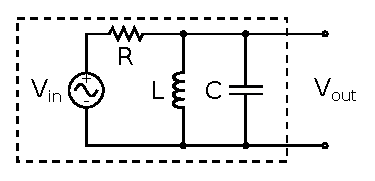
\includegraphics{rlcparallel.eps}
\caption{A Parallel RLC voltage divider.}
\label{fig:rlcparallel}
\end{figure}

In your log book, ...

\begin{enumerate}
\item Derive expressions for the gain, phase angle, and resonant
  frequency of the circuit. You may find Section~\ref{sec:AC} of the
  notes helpful.

\item Pick out an inductor in the 100-1000~$\mu$H range, and then find
  a capacitor you predict will give a resonant frequency in the 10~kHz
  - 100~kHz range.

  \emph{Recall that the angular frequency $\omega$, expressed in
    rad/s, and the frequency $f$, expressed in $Hz$, on the display of
    your function generator are not the same ($\omega = 2\pi f$).}
\end{enumerate}

\subsection*{Experiment}

\emph{You may find that your maximum gain (at resonance) is not
  1, as predicted by your theoretical calculation. Do not
  be alarmed. Just make careful measurements and record them.}

\begin{enumerate}
\item Check that your oscilloscope probes are compensated.

\item Measure the values of $R$ and $C$ with a DMM.

\item Build the circuit in Figure~\ref{fig:rlcparallel}.

\item Set the open-circuit (no load) amplitude of the function
  generator, or the peak-to-peak voltage swing, which ever one your
  oscilloscope gives you automatically, to 10~V as measured with 
  the oscilloscope. Use this value for $V_{in}$ in your gain
  calculations. If you touch the amplitude knob on the function
  generator, be sure to measure the new value of $V_{in}$. 

  \emph{Under load, the signal you measure with the oscilloscope may
    be reduced by voltage division between the load and the output
    resistance of the function generator, in which case it is not
    $V_{in}$.}
  
\item Make measurements to produce gain vs. frequency and phase angle
  vs. frequency plots.

  \emph{Even though the voltage across the function generator under
    load is not $V_{in}$, it has the same phase and can be used to
    measure $\Delta t$ and determine phase angles.}
  
\item Measure the 3~dB points of the circuit. The difference between
  the 3~dB-point frequencies is the band width of the circuit.

  \emph{Since we do not have a way to measure $V_{in}$ directly,
    measure the the 3~dB points by finding the frequencies at which
    $V_{out}$ is reduced by a factor
    $\frac{1}{\sqrt{2}} \approx 0.707$ relative to its maximum
    value.
    (Be aware that its maximum value may not be equal to $V_{in}$!)}
  
\item Use your measured values of $C$ and the resonant frequency of
  the circuit to determine $L$.
\end{enumerate}

\subsection*{Simulation}

At this point, it is likely that you have discovered discrepancies
between your measurements and theoretical predictions. This is at
least partly due to the fact that we did not include the internal
resistance $r_L$ of the inductor or the output resistance $r_{fg}$ of
the function generator in our calculations. Including $r_L$
complicates the algebra significantly. Instead, we will investigate
its impact on the gain with a simulation.

\begin{figure}[h]
\centering
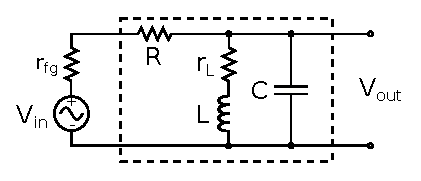
\includegraphics{rlcparallelreal.eps}
\caption{A Parallel RLC voltage divider including the internal
  resistance $r_L$ of the inductor and the output resistance $r_{fg}$
  of the function generator.} 
\label{fig:rlcparallelreal}
\end{figure}

\begin{enumerate}
\item Check the manufacturer's description of your inductor to find
  $r_L$ and the user manual of your function generator for $r_{fg}$.

\item Simulate your design, including $r_L$ and $r_{fg}$ as shown in
Figure~\ref{fig:rlcparallelreal}.  Use a linear AC sweep analysis in
the region of the resonant frequency, and be sure to include lots of
points (1000) so that the point spacing is much smaller than the width
of the resonance.

\item Use the \includegraphics{PSpiceAD_DefineMeasurement.png} button
  to set up a band width calculation
  (\verb+Bandwidth_Bandpass_3dB()+).

\item Use the cursor to determine the resonant frequency.
\end{enumerate}

\subsection*{Products}

Upload to Canvas the PDF of a brief \LaTeX\ report in which you ...
\begin{itemize}
\item Report your measurements of the resistance $R$, capacitance $C$,
  and the inductance $L$.
\item Report your measured value of the resonant frequency of the
  circuit, and compare it with your theoretical prediction.
\item Include as figures ...
  \begin{itemize}
  \item Your measured and simulated gain vs. frequency plots
  \item Your measured phase angle vs. frequency plot
  \item Scans or images of the pages from your log book in which you
    derive expressions for the gain, phase angle, resonant frequency
    of the circuit (neglecting the internal resistance of the inductor
    and the output resistance of the function generator).
  \end{itemize}
\end{itemize}

\end{document}
